%!TEX root = thesis.tex
\chapter{Homeotropic nematics confined in toroids and bent capillaries}

\section{Introduction}
A system with broken reflection symmetry, i.e. it cannot be superimposed onto its reflection using only translations and proper rotations, has a handedness and thus is chiral~\cite{RN175}.
Chirality can have important consequences for a system.
For example, as first shown by Pasteur, optical activity results from broken reflection symmetry, and the handedness of the system determines the direction of the rotation of the polarization of light\cite{RN291}.
In addition, chiral systems can exhibit structural color~\cite{RN308,RN307}, and can even be doped to form microlasers~\cite{RN305,RN306}.
Chiral systems can be formed from chiral building blocks, as in some photonic metamaterials~\cite{RN304}, or chirality can emerge via symmetry breaking in an achiral system\cite{RN294}.
This latter scenario is often studied in nematic liquid crystals where the mesogens are achiral\cite{RN297,RN296,RN298,RN295,RN299,RN193,RN46,RN192,RN191,RN293,RN302}.
Here, the symmetry-breaking is driven by elasticity; if the minimum energy state has a nontrivial twist distortion, then the system is chiral.

This simplest way to break the reflection symmetry is to proscribe it with boundary conditions, as in a twisted nematic cell.
In this scenario, the NLC is confined between two parallel plates with strong planar anchoring on each plate and the anchoring directions on each plate orthogonal to each other; consequently, the boundary conditions require $\mathbf{n}$ to twist by $\pi/2$ along a path between the plates.
Thus, the system has a persistent twist distortion, breaking reflection symmetry.
However, when the twist direction is not specifically set by the boundary, confined liquid crystals can exhibit spontaneous reflection symmetry breaking.
For example, consider a standard bipolar drop with degenerate planar anchoing, as shown schematically in Figure~\ref{f:2-OPMDrops}(A).
If the twist elastic constant $K_{22}$ and bend elastic constant $K_{33}$ are small enough compared to $K_{11}$, the splay elastic constant, the bipolar drop will twist, relieving some some of the splay with the less-costly twist and bend distortions~\cite{RN297,RN296,RN295}.
The criterion governing this instability is called the Williams criterion, $K_{11} > K_{22}+ 0.431 K_{33}$~\cite{RN297}.
Similarly, provided $K_{22}< K^c_{22}$, a NLC confined under homeotropic boundary conditions to a cylindrical capillary will exhibit a twisted escaped-radial (TER) configuration instead of the more common escaped-radial (ER) configuration~\cite{RN192}.

Recent work in our group with NLC confined to capillaries and toroids with degenerate planar boundary conditions have shown that the saddle-splay distortion can also enable a confined NLC to develop chirality~\cite{RN46,RN59,RN293}.
In this case, the saddle splay distortion drives the director at the interface to align along the smallest curvature of the interface according to Eq~\ref{e:2-K24SurfCouple}~\cite{RN59}; as a capillary can be thought of as a torus with an infinite aspect ratio, the criterion for a twisted ground state in both geometries is $K_{24} > K^c_{24}$~\cite{RN24,RN293}.
For a cylindrical capillary, a doubly-twisted state is the ground state if $K^c_{24}>K_{22}$.
However, by increasing the difference between the principle curvatures on the inside of the handle by decreasing $\xi$ and bending the cylinder into a torus, $K^c_{24}$ decreases and the amount of twist in a chiral ground state increases.
This is an example of how geometry can tune chirality.

Inspired by these results in planar-anchored nematic toroids, in this Chapter we consider a 5CB confined to a toroidal droplets under hometropic anchoring.
Despite the fact that the saddle-splay distortion does not enter into the energy minimization for homeotropic nematics, we find spontaneous reflection symmetry breaking and geometrically-controlled chirality.
As with homeotropically-anchored NLC capillaries when $K_{22} < K^c_{22}$~\cite{RN192}, we see that a TER configuration replaces the standard ER configuration.
However, we find TER configurations for $K_{22} > K^c_{22}$; we attribute this to the additional bend distortion introduced when taking a capillary with $\xi \rightarrow \infty$ to a torus with $\xi ~\mathcal(1--10)$.
This additional bend-distortion is relieved by a twist-distortion with a spontaneously-chosen handedness.
In addition, we see that the amount of twist varies inversely with $\xi$, similar to our previous findings in planar anchored toroids.




\section{Escaped radial and twisted escaped radial capillaries}
Consider NLC confined to a cylindrical capillary under homeotropic boundary conditions; in cylindrical coordinates $\{r,\theta,z\}$, we specify the boundary conditions with $\mathbf{n} = \hat{r}$ at the boundary.
Restricting ourselves to a radial director field, $\mathbf{n} = \hat{r}$ everywhere throughout the capillary will yield an $s = +1$ line defect running along $\hat{z}$ at the center of the capillary.
However, recall from Chapter~\ref{c:2} that integer-strength disclination lines are not topologically stable in a 3D NLC.
Similar to line defects in 2D nematics or wall defects in 3D nematics, the singular $s = +1$ distortion can be continuously deformed to form a nonsingular distortion [see Figure~\ref{f:2-Smearing}]~\cite{RN179,RN290,RN289}.
Here, the radial director field ``escapes into the third dimension'', such that  $\mathbf{n}_{z} \neq 0$, hence the name escaped-radial.
In the one-constant approximation, the ER director field is analytically solvable, with $\mathbf{n} = \{\sin(\Omega),0,\cos(\Omega)\}$, where $\Omega = 2 \arctan(r/R)$ gives the director angle measured off of $\hat{z}$, with $R$ the capillary radius~\cite{RN179,RN290}.
Provided $R \gtrsim 0.1$ $\upmu$m, the ER configuration is the ground state solution~\cite{RN194}; the costly splay distortion in the vicinity of the singular line is relieved by a loss-costly bend distortion, with the cost of the bend distortion varying inversely with $R$.

Now starting with an ER configuration in the 1-constant expression, let $K_{22}$ vary while keeping $K_{11} = K_{33} = K$.
When $K_{22} < K^c_{22} \approx 0.27K$~\cite{RN192}, the system can relieve some of the bend and spay distortions in the ER configuration by twisting, yielding the twisted escaped-radial configuration, where now $\mathbf{n}$ has components along $\hat{r}$, $\hat{\theta}$, and $\hat{z}$.
This configuration was first observed using Lyotropic Chromonic Liquid Crystals (LCLC), an aqueous dispersion of plank-like molecules that self-assemble into columnar aggregates; these aggregates then form a nematic at appropriate temperature and concentration~\cite{RN303}.
Since $K_{22} \sim 10^{-1}K$ for LCLC systems, they frequently exhibit spontaneous reflection symmetry breaking~\cite{RN192,RN191,RN293,RN193,RN302}.

The TER and ER configurations can be distinguished by OPM textures.
We fill cylindrical capillaries with 5CB and with an 31.5\% w/w aqueous solution of the LCLC Sunset Yellow (SSY).
To enforce homeotropic anchoring for the 5CB-filled capillaries, we first fill the capillary with $0.1\%$ w/w lecithin in hexane and then let the hexane dry, depositing the lecithin on the inner surface of the capillary.
For the SSY-filled capillaries, we coat the entire capillary with paralyene using chemical vapor deposition.


\subsection{Intensity profile and ratio}
By eye, it is easy to see that the ER and the TER textures are diffferent; this makes sense when we consider the director field in each configuration and its impact on the intensity profile across the capillary.
When the polarizer and analyzer (PA) are aligned along $\hat{z}$ and $\hat{r}$ projected onto the plane of the image, it is easy to see that an OPM texture of an ER capillary should have three regions of extinction corresponding to the edges and  to the center of the capillary.
In these regions, $\mathbf{n}$ is along the PA directions.
Between these three dark regions there are two bright regions, corresponding to locations where $\mathbf{n}$ has components along both $\hat{r}$ and $\hat{z}$.
This dark-bright-dark-bright-dark pattern is the signature of an ER capillary; now plotting the intensity profile across the capillary, we see that there are two clear intensity peaks corresponding the the bright regions, and an intensity minimum in the middle of the profile corresponding to the dark central region.

Conversely, when we look at the OPM texture for a TER configuration, we see that the central region is no longer dark, but now has an appreciable intensity comparable to the two ``bright'' regions flanking the central region.
In a TER configuration, the $\mathbf{n}_{\theta}$ component causes the projection of $\mathbf{n}$ onto the plane of the image to deviate from the PA directions, causing the transmitted intensity in the central region to grow.
Plotting the intensity profile across the capillary, we see that there is still a central minimum surrounded by two peaks; however, the central minimum in the TER configuration is much higher than the central minimum in an ER configuration.
We quantify this difference with an intensity ratio $I_{max}/I_{min}$, with $I_{max}$ the average intensity of the two peaks flanking the central minimum and $I_{min}$ is the intensity of the central minimum; our ER capillaries have $I_{max}/I_{min} \approx 4$ while our TER capillaries have $I_{max}/I_{min} \approx 1$.
We confirm that this phenomenon is not dependent on the LC chosen by comparing with the intensity profile of an ER SSY capillary; while the ground state in a homeotropic SSY capillary is a TER configuration, just after being filled the SSY capillary will have a transient ER configuration that spontaneously breaks reflections symmetry after a few minutes.
As with the ER textures from the 5CB capillaries, $I_{max}/I_{min} \approx 4$ in the ER SSY capillary.




\section{Nematic liquid crystals in toroids}
We make stable toroidal droplets as detailed in Chapter~\ref{c:3}, with 5CB as our inner liquid and an aqueous yield-stress material.
Our yield-stress material for homeotropic nematic toroids is similar to that used in our prior work with planar-anchored nematic toroids~\cite{RN46}, except here, we have replaced the Polyvinyl alcohol used to enforce degenerate planar anchoring with Sodium Dodecyl Sulfate (SDS) to enforce homeotropic anchoring.
The yield-stress material consists of (i) 1.5\% w/w polyacrylamide microgels (Carbopol ETD 2020), (ii) 30\% w/w Ethanol, (iii) 3\% w/w Glycerol, (iv) 25\% w/w 32 mM SDS in ultrapure water, and (v) 40.5\% w/w ultrapure water.
Thus, the final mixture has 8 mM SDS, a concentration that yields strong homeotropic anchoring.
To make the yield-stress material, we mix all the ingredients together, leave the dispersion for $\sim 24$ hrs to allow the Carbopol to hydrate, and then neutralize the mixture using 2M NaOH until the pH$\approx 7$.
Neutralizing the dispersion causes the polyacrylamide microgels to swell, increasing both the yield-stress and the transparency~\cite{RN46,RN47}.

We view our toroidal droplets from the top under both bright-field and with crossed polarizers.
In the OPM textures, the regions where the tube of the torus is along the orientation of the polarizer and analyzer (PA), the intensity pattern has the characteristic dark-light-dark-light-dark profile associated with an ER texture where the cylinder axis is along PA.
However, to quantify the pattern, we need to measure the intensity profile across the tube of the torus.

\subsection{Measuring the intensity profile and aspect ratio}
From the top view, the azimuthal angle in toroidal coordinates, $\{r,\theta,\varphi \}$, corresponds to the polar angle in a set of polar coordinates, $\{p,\varphi \}$, in the image itself.
As $\varphi$ is measured along the central ring of the torus, $p = 0$ corresponds to the center of the central ring of the torus in the image.
We take our intensity profiles across the tube of the torus for a constant $\varphi$ from $p = R_0 - a(\varphi)$ to $p = R_0+ a(\varphi)$, where $R_0$ is the radius of the central ring of the torus and $a$ is the tube radius. m
While for a perfect torus $a = cons't$, our toroidal droplets are not perfectly axisymmetric and thus there is some $\varphi$ dependence.

We find the central ring, $a(\varphi)$, and the intensity profiles with a custom MATLAB script.
From a top-view image, we start by selecting points along the inner and outer contours of the toroid in the image.
We then fit the points on each contour to a circle, giving us the radii $R_{in}$, $R_{out}$ and centers $\mathbf{p}_{in}$, $\mathbf{p}_out$ of the inner and outer contours, respectively.
For a given torus, we can then calculate the aspect ratio $\xi = R_0/a_{av} = (R_{out}+R_{in})/(R_{out}-R_{in})$, with the central ring radius $R_0=(R_{out}+R_{in})/2$ and the average tube radius $a_{av} = (R_{out}-R_{in})/2$.
We also calculate the origin of our polar coordinate system in the image, $\mathbf{p}_0 = (\mathbf{p}_{in}+p_{out})/2$.
For a given $\varphi_0$, we take the intensity contour starting at the inner contour $(\mathbf{p}-\mathbf{p}_{in})^2 = R^2_{in}$ and increasing $p$ until we reach the outer contour $(\mathbf{p}-\mathbf{p}_{out})^2 = R^2_{out}$.
We parameterize each intensity profile with $\rho$, where $\rho = 0$ corresponds to the inner contour and $\rho = 1$ corresponds to the outer contour.


\subsection{Large aspect ratio toroids}
We first look at our larger aspect ratio toroids; the intensity profiles still show a central minimum flanked by two maxima.
However, we find that $I_{max}/I_{min} < 4$, the value for our ER capillaries, with $I_{max}/I_{min}$ increasing and approaching $I_{max}/I_{min} = 4$ as we increase $\xi$.
From this trend, we hypothesize that our toroids have a TER configuration, where the amount of twist depends on $\xi$.


\subsection{Small aspect ratio toroids}
When we look at toroids with smaller $\xi$, we initially see that the intensity pattern has changed to a spiral texture of alternating dark and light regions, no longer resembling the clean dark-bright-dark-bright-dark texture of an ER/TER capillary.
However, when we examine the intensity profile of the spiral textures, we still find qualitative similarities with the intensity profile of an ER/TER configuration, with a central minimum surrounded by two maxima.
In addition, the intensity ratio as a function of $\xi$ for the toroids with a spiral texture is proportional to $\xi$, and the trend overlaps with the intensity ratios from the toroids with a ER/TER configurations.
We turn to simulated OPM textures to investigate the role of twist on the intensity ratio as well as test director configurations that could yield a spiral texture.




\section{Simulating polarized optical microscopy textures for twisted escaped radial director configurations}
\subsection{Jones Calculus and simulation details}
Jones Calculus is a method to describe and propagate polarized light through a birefringent material~\cite{RN232}.
The state of the polarized light is characterized by decomposing the electric field in the plane of polarization using a 2-dimensional Jones vector while neglecting the time dependence of the electric field.
We can neglect the time dependence because while the electric field oscillates with time, the polarization state does not.
For example, allowing $\hat{x}$ to be horizontal, $\hat{y}$ to be vertical, and $\hat{k}_0 = \hat{z}$ the direction of the wavevector of the polarized incident light, we can write the normalized electric field as:
\begin{align}
\hat{E} &=  \hat{x}E_x e^{i \phi _x} + \hat{y} E_y e^{i \phi _y}\\  &= e^{i \phi _x} \left[ \begin{array}{c} E_x \\E_y e^{i(\phi _y - \phi _x)}      \end{array} \right]. \label{e:4-jonesdecomp}
\end{align}
Thus, the Jones vector for a horizontal polarization state, a $+45$ degree polarization state, and a right-hand circular polarization state can be written as $(1,0)$, $(1,1)/\sqrt(2)$, and $(1,i)/\sqrt(2)$, respectively.
We have normalized the Jones vectors, removing the absolute phase prefactor $e^{i \phi _x}$ from equation \ref{e:4-jonesdecomp} as the polarization state is dependent on neither the absolute phase nor the magnitude of the vector.
Note, in particular, that the the Jones vector for the right-hand circularly polarized light gives the normalized field $\hat{E} = \hat{x}E_x e^{i \phi _x} + \hat{y} E_y e^{i( \phi _x+\pi)}$, as we would expect.

In order to propagate a polarization state through an optical element (e.g. half-wave plate, phase retarder), we write each component of the Jones vector representing the transformed state $\vec{E_t}$ as a linear combination of the components of the Jones vector representing the initial state $\vec{E_i} = E_{ix}\hat{x}+E_{iy}\hat{y}$:
\begin{align}
\vec{E}_t = \left [ \begin{array}{c} \vec{E}_{tx} \\ \vec{E}_{ty} \end{array} \right ] &= \left [ \begin{array}{c} A \vec{E}_{ix} + B \vec{E}_{iy} \\ C \vec{E}_{ix}+ D \vec{E}_{ty} \end{array} \right ] \nonumber \\
&= \left [ \begin{array}{cc} A & B \\C & D \end{array} \right ]\left [ \begin{array}{c} \vec{E}_{ix} \\ \vec{E}_{iy} \end{array} \right ] = \bar{\bar{\Theta}} \vec{E}_i ,
\end{align}
where $\dbar{\Theta}$ is is our transformation operator, which can be written as a $2 \times 2$ Jones matrix.
To propagate a Jones vector through multiple optical elements, the Jones matrix for each element is applied to the initial Jones vector sequentially.
For a series of $N$ elements:
\begin{equation}
\vec{E}_t = \dbar{\Theta}_N \dbar{\Theta}_{N-1} \cdots \dbar{\Theta}_2 \dbar{\Theta}_1\, \vec{E}_i = \prod^N_{j=1} \dbar{\Theta}_j \vec{E}_i = \dbar{\vartheta} \vec{E}_i,
\end{equation}
where $\dbar{\vartheta}$ is the operator representing the Jones matrix for the entire system.
A list of some common optical elements represented as Jones Matrices in the $x-y$ basis can be seen in Table~\ref{t:4-jmats}.
\begin{table}
\caption{sdf}
\begin{tabular}{|c|c|}
\hline
{\bf Optical Element} & {\bf Jones Matrix} \\ \hline \hline
Linear polarizer with axis of transmission horizontal & $\begin{pmatrix}1 & 0 \\ 0 & 0 \end{pmatrix}$ \\ \hline
Linear polarizer with axis of transmission vertical &$\begin{pmatrix}0 & 0 \\ 0 & 1 \end{pmatrix}$ \\ \hline
Linear polarizer with axis of transmission at $\pm 45^o$ with the horizontal &$\frac{1}{2} \begin{pmatrix}1 & \pm 1 \\ \pm 1 & 1\end{pmatrix}$ \\ \hline
Right/Left circular polarizer & $\frac{1}{2} \begin{pmatrix}
1 & \pm i \\ \mp i & 1
\end{pmatrix}$ \\
\hline
\end{tabular}\label{t:4-jmats}
\end{table}

For a general phase retarder with the fast axis along $\hat{y}$, the transformation operator is written as~\cite{RN232}:
\begin{equation}\label{e:4-fastaxisy}
\dbar{\Theta} = \begin{bmatrix}e^{i \phi_x} & 0 \\ 0 & e^{i \phi_y} \end{bmatrix}.
\end{equation}
When the orientation of the fast axis is not along $\hat{y}$, we use a rotation matrix to rotate $\vec{E}_i$ along $\hat{y}$ so we can use equation \ref{e:4-fastaxisy}; we undo our initial rotation with a second rotation matrix afterwards~\fxnote{Microscope textures of nematic droplets}:
\begin{equation} \label{e:4-jones_decouple}
\vec{E}_t = \dbar{R}(-\alpha)\dbar{\Theta} \dbar{R}(\alpha)\,\vec{E}_i,
\end{equation}
where $\dbar{R}(\alpha) = \begin{bmatrix} \cos \alpha & -\sin \alpha \\ \sin \alpha & \cos \alpha \end{bmatrix}$
is the rotation matrix for an angle $\alpha$ measured with respect to the x-axis.
This approach simplifies calculations for a series of optical elements.

Since we wish to simulate the POM texture of a continuous volume with a given nematic director field, we first need to discretize the continuous nematic volume into cubic volume elements, or voxels, of side $\Delta$.
If $\Delta$ is small enough such that the local director $\hat{n}_i$ for each voxel $ i \;\epsilon \, [1,N]$ can be treated as constant throughout the voxel, then each voxel can be treated as a phase retarder with the associated Jones Matrix and orientation given by its $\hat{n}_i$.
In this way, we are able to treat a continuous nematic volume as a collection of independent optical elements.

As the extraordinary index of refraction of a birefringent uniaxial material depends on the angle $\gamma$ between $\hat{n}$ and $\vec{k}_0$ according to $n_e(\gamma) = n_o n_E/\sqrt{n^2_o \sin^2\gamma+n_E^2 \cos^2 \gamma}$ with $n_o$ the ordinary index of refraction and $n_E$ the extraordinary index of refraction for $\gamma = \pi/2$, we can write the Jones Matrix for the $i^{th}$ voxel with the fast axis along $\hat{y}$ as:
\begin{equation}
\dbar{\Theta}_i  =  \begin{bmatrix}e^{i(n_o2 \pi \frac{\Delta}{\lambda})} & 0 \\ 0 & e^{i (n_e(\gamma_i)2 \pi \frac{\Delta}{\lambda})} \end{bmatrix},
\end{equation}
where $\lambda$ is the wavelength of the light and where we have set $\hat{k}_0=\hat{z}$ such that the plane of polarization is in the $x-y$ plane.
To use the formalism underlying Eq.~\ref{e:4-jones_decouple}, we need the angle between $\vec{k}_0$ and $\hat{n}_i$, $\gamma_i$, and the angle between the projection of $\hat{n}_i$ onto the $x-y$ plane and the x-axis, $\alpha_i$.
Note that the angle between the average director of the overall nematic configuration $\hat{n}_d$ and $\vec{k}_0$ is $\theta_0$, and the angle between the projection of $\hat{n}_d$ onto the x-y plane and the x-axis is the orientation $\alpha_0$.
We use these two angles to control the orientation of the nematic configuration with respect to $\vec{k}_0$ such that we can simulate POM textures for different views of the nematic configuration.
In addition, we change the polarizer orientation by changing the orientation of the incident polarization, given by $\vec{E}_p$.
The angles used to describe the local director as well as the angles used to describe the orientation of the entire nematic configuration are shown in Figure~\fxnote{f:4-generalcoords}(A).
\begin{figure}
\centering
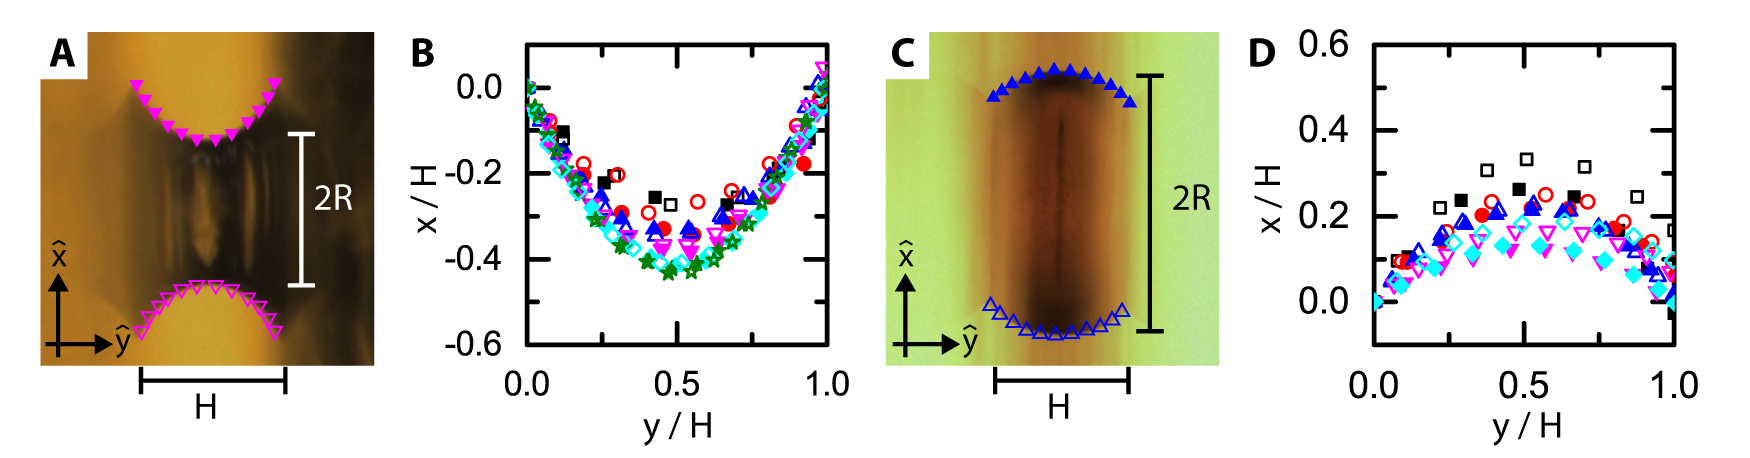
\includegraphics{figures/C5/Ch5-Figs_ShapeContour.png}
\caption{Symbols and coordinates used in simulating POM droplet textures.
(A), Relevant angles used in all simulations, where $\hat{n}_d$ is the droplet director, $\hat{n}_i$ is the local director, $\vec{k}_0$ is the incident wave vector, and $\vec{E}_p$ gives the orientation of the polarizer.
(B), Breakdown of POM simulation parameters in a spherical geometry, where $\vec{\rho}$ is the position vector in the final image and $\Delta$ is the thickness of the voxels used in the simulation.}\label{f:4-generalcoords}
\end{figure}

To find the intensity at a given point $I(\vec{\rho})$ in the final simulated POM texture, $\vec{E}_p$ is propagated along the ray $\vec{k}_0$ passing through $\vec{\rho}$.
To accomplish this, the Jones Matrix and rotation matrices for every voxel encountered by $\vec{k}_0$ are applied to the initial polarization state to produce the final polarization state of the light leaving the nematic volume.
A schematic of this process for a spherical nematic volume can be seen in Figure \ref{f:4-generalcoords}(B), where $I(\vec{\rho})$ is the magnitude squared of the final polarization state after it has passed through the analyzer.
Writing $I(\vec{\rho})$ in terms of $\dbar{\Theta}$ and $\dbar{R}(\alpha)$:
\begin{align}
I(\vec{\rho}) &= |\dbar{\Theta}_A \dbar{R}(\vec{\rho})_A\, \dbar{\vartheta}(\vec{\rho}) \, \vec{E}_P|^2, \, \label{e:4-Intensity} \\
 & \quad\quad\textrm{where}\\
        & \dbar{\vartheta}(\vec{\rho}) =  \prod_{i = 1}^{N(\vec{\rho})}\!\dbar{R}(-\alpha(\vec{\rho})_i) \dbar{\Theta}(\vec{\rho})_i \dbar{R}(\alpha(\vec{\rho})_i)\,, \label{e:4-general_operator_one}
\end{align}
and $\dbar{\Theta}_A \dbar{R}(\vec{\rho})_A$ is the operator and associated rotation representing the analyzer.
Taking advantage of the associative property of matrix multiplication and the fact that the product of two rotation matrices is the rotation matrix of the sum of the angles, we can re-write Eq.~\ref{e:4-general_operator_one} as:
\begin{equation}
\dbar{\vartheta}(\vec{\rho}) =  \prod_{i = 1}^{N(\vec{\rho})}\!\dbar{\Theta}(\vec{\rho})_i \dbar{R}(\alpha(\vec{\rho})_i-\alpha(\vec{\rho})_{i-1})\,
\end{equation}

Therefore, the overall process to simulate a POM texture from a given director field is: (1) discretize the volume into voxels such that the local director for each voxel can be considered constant, (2) use the local director to calculate the angles $\gamma$ and $\alpha$ for each voxel, (3) use $\gamma$ and $\alpha$ to determine the Jones Matrix and rotation matrix associated with each voxel, (4) propagate the inital polarization state through the series of rotation matrices and Jones Matrices, and (5) pass the final polarization state through the analyzer and square the magnitude of the output to obtain the final intensity map.
\begin{figure}
\centering
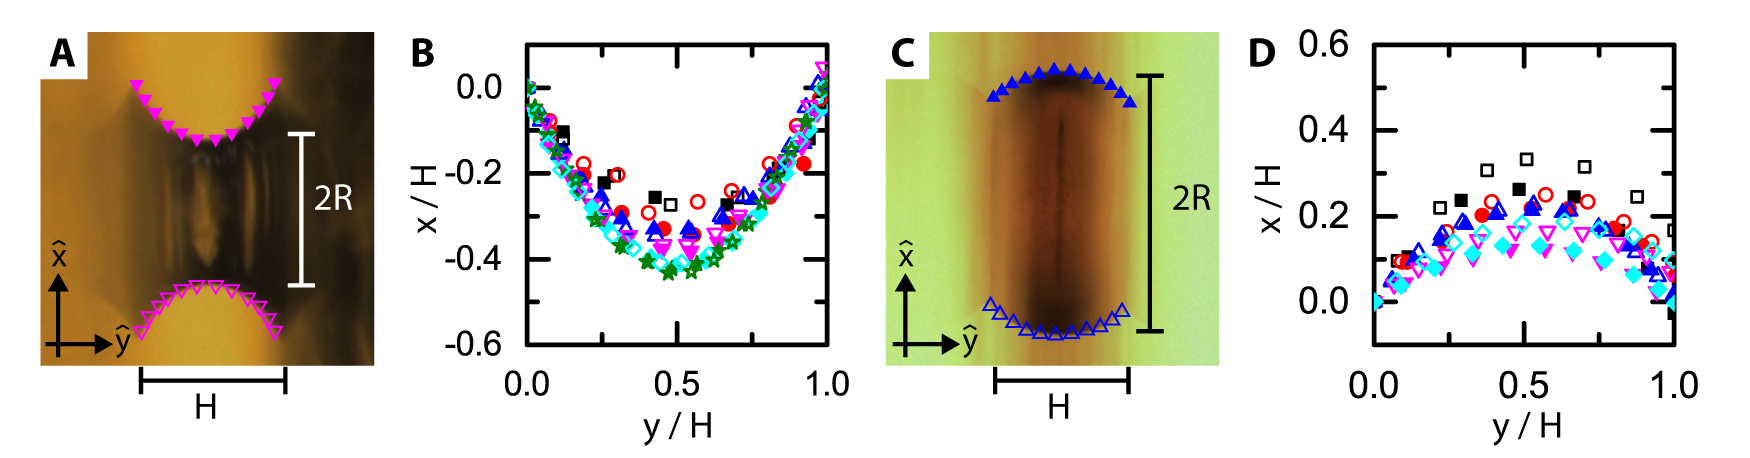
\includegraphics{figures/C5/Ch5-Figs_ShapeContour.png}
\caption{Simulated and experimental POM textures for (A--D) radial droplets, (E--J) bipolar droplets, and (K--P) twisted bipolar droplets.
For the radial droplets, (A) is a our simulation, (B,D) are a grayscale and color experimental image, respectively, and (C) is a simulation image from Ref.~{ondris1991microscope}.
For the bipolar and twisted bipolar  droplets, (E--F) and (K--M) are oriented with the bipole aligned parallel to the analyzer direction while (H--J) and (N--P) have the bipole rotated 15 degrees CCW from the analyzer direction. (E,H,K,N) are our simulated images, (F,I,L,O) are experimental images, and (G,J,M,P) are simulated textures from the literature.
(G,J) are from Ref.~{ondris1991microscope}, (L,M,O,P) are from Ref.~\cite{RN193}.
Scale bar is 20 $\upmu$m in all images.
Images from Ref.~{ondris1991microscope} and Ref~\cite{RN193} reproduced with permission from {\bf GET PERMISSION}
}\label{f:4-spherecomparison}
\end{figure}

\subsection{Validation using spherical droplets}
To test this method, we simulated POM textures for the well-studied radial, bipolar, and twisted-bipolar director fields in spherical geometries.
For a radial director field we used $\hat{n}_r = (x,y,z)/\sqrt{x^2+y^2+z^2}$~\cite{RN232}.
A simulated texture of a 40 $\upmu$m diameter sphere calculated using $20$ evenly spaced wavelengths between $400$~nm and $700$~nm is shown in Figure~\ref{f:4-spherecomparison}(A).
We compare our simulated image both with a grayscale experimental image of a 5CB droplet in water with 8 mM SDS and with another simulated texture of a $10$ $\upmu$m diameter sphere from~\fxnote{ondris1991microscope}.
These are shown in Figure~\ref{f:4-spherecomparison}(B,C), respectively.
The image in Figure~\ref{f:4-spherecomparison}(B) was converted to grayscale from the RGB image in Figure~\ref{f:4-spherecomparison}(D) using MATLAB's \texttt{rgb2gray} algorithm: $gray = 0.299 \textrm{R} + 0.587 \textrm{G} + 0.114 \textrm{B}$.
The conversion was done to better compare the simulated and experimental textures.
Note the agreement between our simulated image and the grayscale experimental texture; both show four dark wedge-shaped brushes that begin in the center of the droplet and extend to the edges.
The bright portions also have roughly homogeneous intensity.
However, the experimental image is brighter in the center than our simulated image.
We attribute this difference to the defect not being in the focal plane in the experimental image; our simulated image does not take into account focus effects.
In addition, note how the bright portions of Figure~\ref{f:4-spherecomparison}(C) do not have an even intensity.
This is due to the size of the droplet simulated.

For a bipolar director we use $\hat{n}_b = \nabla \psi/|\nabla \psi|$, where
\begin{align}
\psi =& \frac{1}{\sqrt{(x-p_x)^2+(y-p_y)^2+(z-p_z)^2}} \nonumber \\
      -& \frac{1}{\sqrt{(x+p_x)^2+(y+p_y)^2+(z+p_z)^2}}, \label{e:4-bipolar_pot}
\end{align}
$\vec{p} = R(\sin \theta_0\cos\alpha_0,\sin \theta_0\sin\alpha_0,\cos\theta_0) $, with $R$ the sphere radius.
The simulated bipolar POM texture of a 40 $\mu$m diameter sphere for this director field using 20 evenly spaced wavelengths between $400$ nm and $700$ nm for $\theta_0 = \pi/2$ and either $\alpha_0 = 0$ or $\alpha_0 = \pi/12$, as shown in Figure~\ref{f:4-spherecomparison}(E,H), respectively.
Corresponding experimental images of a 5CB droplet in water with $1\%$ Polyvinyl alcohol, enforcing tangential anchoring, as well as simulated images of a 40 $\upmu$m diameter sphere from Ref.~\fxnote{ondris1991microscope} are shown in Figure~\ref{f:4-spherecomparison}(F,I) and Figure~\ref{f:4-spherecomparison}(G,J), respectively.
All six images exhibit remarkable agreement.
Note how Figure~\ref{f:4-spherecomparison}(E--G) all have four bright portions at the edge of the droplet and how the bright regions show a greater horizontal separation than a vertical separation.
Note also how the central region is completely dark.
When the droplet orientation changes by $\pi/12$ as seen in Figure \ref{f:4-spherecomparison}(H--J), the central region in all three textures ceases being completely dark and begins to connect the upper-left and lower-right bright regions.

For a twisted bipolar director $\hat{n}_{tb}$, we follow Ref.~\cite{RN177} and use:
\begin{equation}
\hat{n}_{tb} = \hat{n}_{b}\cos\tau +\hat{n}_{c}\sin\tau,
\end{equation}
where the concentric director is $\hat{n}_{c} = (\sin \phi,\cos \phi,0)$, with $\phi$ the polar angle measured off of the x-axis.
$\hat{n}_b$ is the bipolar director derived from the normalized gradient of Eq.~\ref{e:4-bipolar_pot}, and $\tau = \tau_0\sqrt{x^2+y^2}/\sqrt{R^2-z^2}$ is a twist angle varying from $\tau=\tau_0$ at the surface of the sphere to $\tau=0$ at the bipole axis~\cite{RN177}.
Instead of generating POM textures with different $\alpha_0$ and a fixed polarizer and analyzer orientation as with the bipolar POM textures, here we keep $\alpha_0=0$ and vary the polarizer and the analyzer orientation to generate different views.
This makes the computation easier to perform. Our simulated twisted bipolar POM textures seen in Figure~\ref{f:4-spherecomparison}(K,N) were produced for a 50 $\upmu$m diameter sphere with a single wavelength at $\lambda = 650$~nm.
The simulated twisted bipolar images from Ref.~\cite{RN193} were also produced for a similar sphere with $\lambda = 650$~nm, as seen in Figure~\ref{f:4-spherecomparison}(M,P).
The experimental images of $\sim 40$ $\upmu$m diameter droplets imaged using $\lambda \sim 650$~nm from Ref.~\cite{RN193}are shown in Figure~\ref{f:4-spherecomparison}(L,O).
As with the bipolar droplets, the six twisted bipolar textures also show remarkable agreement.
Note how the number and position of the alternating bright and dark regions in Figure~\ref{f:4-spherecomparison}(K--M) and Figure~\ref{f:4-spherecomparison}(N--P) are the same.
In addition, note that while the central region in the bipolar drops in Figure~\ref{f:4-spherecomparison}(E--G) is dark, the addition of a twist in the director field about the horizontal axis causes the central region in the twisted bipolar textures in Figure~\ref{f:4-spherecomparison}(K--M) to be bright.
Even though 20 wavelengths were used for the bipolar textures and only a single wavelength was used for the twisted bipolar textures, this is a valid comparison to make.
Using more or fewer wavelengths for the bipolar texture would not brighten the center and using more wavelengths in the twisted bipolar texture would not darken the central region.


\subsection{Planar-anchored nematic toroids}
\subsection{Comparison with homeoetropic-anchored nematic toroids}
\subsection{Intensity ratio as a function of twist parameter}

\section{Nematic liquid crystals in bent capillaries}
\subsection{Making bent capillaries}
\subsection{Measuring planar curvature}
\subsection{Measuring the intensity profile}
\subsection{Comparison with toroids}

\section{Conclusions}
